\documentclass[UTF8]{ctexbeamer}

\usetheme{Boadilla}

\usecolortheme{rose}

\usepackage{graphicx}
\usepackage{color}
\usepackage{tikz}
\usepackage{xcolor}
\usepackage{pgfplots}
\usepackage{listings}
\usepackage{amsmath}

\pgfplotsset{width=7cm,compat=1.6}
\usefonttheme[onlymath]{serif}

\newfontfamily\courier{Courier New}
\lstset{linewidth=1.1\textwidth,
	numbers=left,
	basicstyle=\small\courier,
	numberstyle=\tiny\courier,
	keywordstyle=\color{blue}\courier,
	commentstyle=\it\color[cmyk]{1,0,1,0}\courier, 
	stringstyle=\it\color[RGB]{128,0,0}\courier,
	breaklines,
	extendedchars=false, 
	xleftmargin=2em,xrightmargin=2em, aboveskip=1em,
	tabsize=4, 
	basicstyle=\small\courier
}

\tikzstyle{myBlock}=[draw, fill=blue!30!white, minimum size=0.5in, node distance=2.25in]
\usetikzlibrary{arrows.meta}
\tikzstyle{myPath} = [-{Latex[length=2mm,width=2mm]}, line width=0.4mm]


\begin{document}

\title{多项式乘法与快速傅里叶变换}
\author{\songti 于海鑫}
\institute{2017211240}

\date{\today}

\frame{\titlepage}

\section{多项式}
\begin{frame}
\frametitle{多项式}
\begin{itemize}
  \item 以 $x$ 为变量的\textbf{多项式}定义在数域 $F$ 上,将函数
  $$ A(x) = a_{n-1}x^{n - 1} + \cdots + a_2 x^2 + a_1 x^1 + a_0$$
  表示为形式和 $ A(x) = \sum_{i = 0}^{n - 1} a_i x^i$ 的形式
  \item $a_0, a_1, \cdots , a_{n-1}$ 被称为多项式的\textbf{系数}
  \item 如果 $A(x)$ 的最高次的非零系数是 $a_k$,则称 $A(x)$ 的\textbf{次数}为 $k$
  \item 任何严格大于多项式的次数的整数都是该多项式的\textbf{次数界}
\end{itemize}
\end{frame}

\begin{frame}
    \frametitle{多项式的表示}
    \begin{block}{系数表达}
        对于多项式 $A(x)$ ,其\textbf{系数表达}为由其系数组成的向量
        $$\vec{a} = (a_0, a_1, \cdots, a_{n_1})$$
    \end{block}
    \begin{block}{点值表达}
        次数界为 $n$ 的多项式 $A(x)$ 的\textbf{点值表达}为 $n$ 个点值对
        构成的集合 $$\{ (x_0, y_0),  (x_1, y_1), \cdots, (x_{n-1}, y_{n-1})\}$$
        \begin{center}
            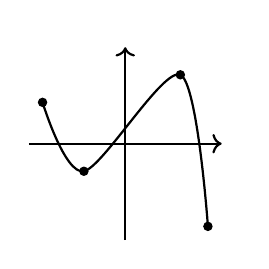
\begin{tikzpicture}[scale=.35]
                \draw[thick,->] (-3.5,0) -- (3.5,0) node[anchor=north west] {};
                \draw[thick,->] (0,-3.5) -- (0,3.5) node[anchor=south east] {};
                \draw[thick] plot[smooth] coordinates  {(-3,1.5) (-1.5,-1) (2,2.5) (3,-3)};
                \foreach \Point/\PointLabel in {(-3,1.5)/, (-1.5,-1)/, (2,2.5)/, (3,-3)/}
                \draw[fill=black] \Point circle (0.15) node[above right] {$\PointLabel$};
            \end{tikzpicture}
        \end{center}
    \end{block}
\end{frame}

\begin{frame}
    \frametitle{举例}
    对于多项式:
    $$ A(x) = x^3 + x^2 + 1 $$

    \begin{itemize}
        \item $A(x)$ 的系数为 $3$
        \item $A(x)$ 的次数界为 $4, 5, \cdots$ 等全部大于 $3$ 的数
        \item $A(x)$ 的系数表示为 $ (1, 1, 0, 1)$
        \item $A(x)$ 的一个点值表达为 $\{ (-1, 1), (0, 1), (1, 3), (2, 13) \}$
    \end{itemize}
\end{frame}

\begin{frame}
    \frametitle{表达形式的转换}
    \begin{block}{系数表达 $\Rightarrow$ 点值表达 aka 求值}
        直接对选取的点进行求值即可,时间复杂度为 $\textcolor{red}{\Theta(n^2)}$
    \end{block}
    \begin{block}{点值表达 $\Rightarrow$ 系数表达 aka 插值}
        对于给定的点值对集合 $\{ (x_0, y_0), \cdots, (x_{n-1}, y_{n-1})\}$
        使用\textbf{拉格朗日公式}
        $$A(x) = \sum_{k = 0}^{n - 1} y_k \frac{\prod_{j \neq k}(x - x_j)}{\prod_{j \neq k}(x_k - x_j)}$$
        即可求出 $A(x)$ 的系数表达。时间复杂度为 $\textcolor{red}{\Theta(n^2)}$。
    \end{block}
\end{frame}

\section{多项式的乘法}

\begin{frame}
    \frametitle{多项式的乘法}
    对于多项式乘法,如果$A(x). B(x)$均为次数界为 $n$ 的多项式,
    则它们的\textbf{乘积} $C(x)$ 是一个次数界为 $2n - 1$ 的多项式,
    对于任一属于多项式定义域的$x$,都有$C(x) = A(x)B(x)$
\end{frame}

\begin{frame}
    \frametitle{多项式的乘法}
    当多项式为\textbf{系数}表达时,其乘积的计算方法相当简单,对于表示为
    $$\vec{a} = (a_0, a_1, \cdots, a_{n-1})$$
    $$\vec{b} = (b_0, b_1, \cdots, b_{n-1})$$
    的多项式$A(x). B(x)$,其乘积$C(x)$的系数表达为:
    $$\vec{b} = (c_0, c_1, \cdots, c_{2n-1})$$
    其中
    $$c_i = \sum_{j = 0}^{i} a_j b_{i - j} \qquad \Rightarrow \textcolor{red}{\Theta(n^2)}$$
    \begin{block}{}
        $\vec{c}$ 被称为 $\vec{a}$ 和 $\vec{b}$ 的卷积,记为
        $\vec{c} = \vec{a} \otimes \vec{b}$
    \end{block}
\end{frame}

\begin{frame}
    \frametitle{多项式的乘法}
    当多项式为\textbf{点值}表达时,对于任一点$x_k$,由都有$C(x_k) = A(x_k)B(x_k)$。
    同时注意到
    $$degree(C) = degree(A) + degree(B)$$
    因此当 $A(x), B(x)$ 的点值表达分别为(注意对于$A(x),B(x)$需要$2n$个点值对)
    $$A:\{ (x_0, y_0), \cdots, (x_{2n-1}, y_{2n-1})\}$$
    $$B:\{ (x_0, y_0'), \cdots, (x_{2n-1}, y_{2n-1}')\}$$
    时,$C(x)$的点值表达应为:
    $$C:\{ (x_0, z_0), \cdots, (x_{2n-1}, z_{2n-1})\}$$
    其中
    $$z_i = y_i y_i' \qquad \Rightarrow \textcolor{green}{\Theta(n)}$$
\end{frame}


\begin{frame}
    \frametitle{多项式的乘法}

\begin{figure}[H]
\centering
\begin{tikzpicture}
   \node[myBlock] (v) {\begin{tabular}{c} $\vec{a} = (a_0, a_1, \cdots, a_{n-1})$ \\ $\vec{b} = (b_0, b_1, \cdots, b_{n-1})$ \end{tabular}};
   \node[myBlock] (p) [right of=v] {$\vec{c} = (c_0, c_1, \cdots, c_{2n-1})$};
   \node[myBlock] (s) [below of=v] {\begin{tabular}{c} $A(x_0), B(x_0)$ \\ $A(x_1), B(x_1)$ \\ $\cdots$ \\ $A(x_{2n-1}), B(x_{2n-1})$ \end{tabular}};
   \node[myBlock] (b) [right of=s] {\begin{tabular}{c} $C(x_0)$ \\ $C(x_1)$ \\ $\cdots$ \\ $C(x_{2n-1})$ \end{tabular}};

    \draw[myPath] (v) -- (p) node [midway, above] {$\otimes$, $\textcolor{red}{\Theta(n^2)}$};
   \draw[myPath] (s) -- (b) node [midway, above] {$\times$, $\textcolor{green}{\Theta(n)}$};
   \draw[myPath] (v) -- (s) node [midway, left] {求值, $\textcolor{red}{\Theta(n^2)}$};
   \draw[myPath] (b) -- (p) node [midway, left] {插值, $\textcolor{red}{\Theta(n^2)}$};

\end{tikzpicture}
\label{fig:block_diagram}
\end{figure}

\end{frame}

\section{快速傅里叶变换}

\begin{frame}
    \frametitle{Can we do better?}
    使用\textbf{快速傅里叶变换},我们可以在
    $\textcolor{blue}{\Theta(n \log n)}$ 的时间复杂度下
    完成两种表示形式的转换
 
    此时我们可以在 $\textcolor{blue}{\Theta(n \log n)}$
    的时间复杂度内计算多项式的乘积
\end{frame}

\begin{frame}
    \frametitle{傅里叶变换}
    \begin{itemize}
        \item 有史以来最伟大、最深刻的发现之一
        \item 将时域信号转换为频域信号
    \end{itemize}
    \begin{figure}
        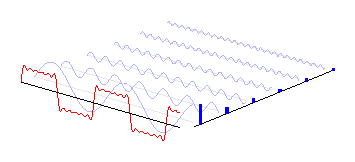
\includegraphics[width= 0.8\linewidth]{ft.pdf}
     \end{figure}
\end{frame}

\begin{frame}
    \frametitle{N 次单位根}
    \begin{block}{}
        称方程 $\omega^n = 1$ 在 $\mathbb{C}$ 上的 n 个解
        $$\omega_k = \exp^{\frac{2k\pi i}{n}} = \cos(\frac{2\pi k}{n}) + i \sin(\frac{2\pi k}{n})$$
        为 \textbf{n 次单位根}
    \end{block}
    显然,N 次单位根有如下性质:
    \begin{itemize}
        \item $\omega_{dn}^{dk} = \omega_{n}^{k}$ (Cancellation Lemma)
        \item 当 $n$ 为偶数时,$(\omega_n^{k + n/2})^2 = (\omega_n^k)^2$ (Halving Lemma)
        \item 当 $n \geq 1$ 时,对于 $k \neq 0$ 且 $k$ 不被 $n$ 整除,有 
        $\sum_{j = 0}^{n - 1} (\omega_n^k)^j = 0$ (Summation Lemma)
    \end{itemize}
    \begin{center}
        \sout{证明留做习题}
    \end{center}
\end{frame}

\begin{frame}
    \frametitle{离散傅里叶变换(DFT)}
    可用于求次数界为 $n$ 的多项式 $A(x)$ 在
    $(\omega_n^{0}, \omega_n^{1}, \cdots, \omega_n^{n - 1})$
    处进行求值。为了简化问题,在这里我们假设
    \begin{itemize}
        \item $n$ 是 2 的幂
        \item A(x) 被表示为系数向量 $\vec{a} = (a_0, a_1, \cdots, a_{n-1})$
    \end{itemize}
    我们定义,对于上文所述多项式 $A(x)$,向量 $\vec{y} = (y_0, y_1, \cdots, y_{n-1})$ 被称为
    系数向量的\textbf{离散傅里叶变换},其中
    $$y_k = A(\omega_n^k) = \sum_{i = 0}^{n-1} a_i \omega_n^{ki}$$
    可记
    $$\vec{y} = DFT_n(\vec{a}) \qquad \Rightarrow \textcolor{red}{\Theta(n^2)}$$
\end{frame}

\begin{frame}
    \frametitle{快速傅里叶变换(FFT)}
    \centering ``The most important numerical algorithm of our lifetime'' \\ by G. Strang, 1994
\end{frame}

\begin{frame}
    \frametitle{分而治之}
    $$A^{[0]}(x) = a_0 + a_2 x + a_4 x^2 + \cdots + a_{n-2} x^{\frac{n}{2} - 1}$$
    $$A^{[1]}(x) = a_1 + a_3 x + a_5 x^2 + \cdots + a_{n-1} x^{\frac{n}{2} - 1}$$
    $$A(x) = A^{[0]}(x^2) + xA^{[1]}(x^2)$$
    $$T(n) = 2T(\frac{n}{2}) + \Theta(n) \qquad \Rightarrow \textcolor{blue}{\Theta(n \log n)}$$
\end{frame}

\begin{frame}
    \frametitle{正确性证明}
    对于 $y_0, y_1, \cdots\, y_{n/2 - 1}$ 有
    \begin{displaymath} 
        \begin{aligned}	 
         y_k & = y_k^{[0]} + \omega_n^k y_k^{[1]} \\
         & = A^{[0]}(\omega_n^{2k}) + \omega_n^k A^{[1]}(\omega_n^{2k}) \\
         & = A(\omega_n^k)
         \end{aligned}
    \end{displaymath}
    对于 $y_{n/2}, y_{n/2 + 1}, \cdots\, y_{n - 1}$ 有
    \begin{displaymath} 
        \begin{aligned}	 
         y_{k + n/2} & = y_k^{[0]} - \omega_n^k y_k^{[1]} \\
         & = y_k^{[0]} + \omega_n^{k + n/2} y_k^{[1]} \\
         & = A^{[0]}(\omega_n^{2k}) + \omega_n^{k + n/2} A^{[1]}(\omega_n^{2k}) \\
         & = A^{[0]}(\omega_n^{2k + n}) + \omega_n^{k + n/2} A^{[1]}(\omega_n^{2k + n}) \\
         & = A(\omega_n^{k + n/2})
         \end{aligned}
    \end{displaymath}
\end{frame}

\begin{frame}
    \frametitle{逆 DFT}
    如果 $y = DFT_n(y)$ 则可以记 $a = DFT^{-1}_n(y)$
    
    通过对 FFT 进行以下修改,我们可以在 $\textcolor{blue}{\Theta(n \log n)}$ 的
    时间复杂度下计算 $DFT_n^{-1}$:
    \begin{itemize}
        \item $a$ 和 $y$ 的位置互换
        \item $\omega_n$ 替换为 $\omega_n^{-1}$
        \item 结果除以 $n$
    \end{itemize}
\end{frame}

\begin{frame}
    \frametitle{多项式的乘法}
\begin{figure}[H]
\centering
\begin{tikzpicture}
   \node[myBlock] (v) {\begin{tabular}{c} $\vec{a} = (a_0, a_1, \cdots, a_{n-1})$ \\ $\vec{b} = (b_0, b_1, \cdots, b_{n-1})$ \end{tabular}};
   \node[myBlock] (p) [right of=v] {$\vec{c} = (c_0, c_1, \cdots, c_{2n-1})$};
   \node[myBlock] (s) [below of=v] {\begin{tabular}{c} $A(x_0), B(x_0)$ \\ $A(x_1), B(x_1)$ \\ $\cdots$ \\ $A(x_{2n-1}), B(x_{2n-1})$ \end{tabular}};
   \node[myBlock] (b) [right of=s] {\begin{tabular}{c} $C(x_0)$ \\ $C(x_1)$ \\ $\cdots$ \\ $C(x_{2n-1})$ \end{tabular}};

   % Draw line between each of the blocks
   \draw[myPath] (v) -- (p) node [midway, above] {$\otimes$, $\textcolor{red}{\Theta(n^2)}$};
   \draw[myPath] (s) -- (b) node [midway, above] {$\times$, $\textcolor{green}{\Theta(n)}$};
   \draw[myPath] (v) -- (s) node [midway, left] {FFT, $\textcolor{blue}{\Theta(n \log n)}$};
   \draw[myPath] (b) -- (p) node [midway, left] {逆FFT, $\textcolor{blue}{\Theta(n \log n)}$};

\end{tikzpicture}
\label{fig:block_diagram_2}
\end{figure}

\end{frame}

\begin{frame}
    \frametitle{卷积定理}
    对任何长度为 $n$ 的向量 $\vec{a}$ 和 $\vec{b}$,有
    $$\vec{a} \otimes \vec{b} = DFT_{2n}^{-1}(DFT_{2n}(\vec{a}) · DFT_{2n}{\vec{b}})$$
\end{frame}

\section{代码实现}

\begin{frame}[fragile]
    \frametitle{代码实现:N次单位根}
    \begin{lstlisting}[language=Python]
from cmath import exp
from math import pi


class NthRootOfUnity:
    def __init__(self, n, k=1):
        self.k = k
        self.n = n

    def __pow__(self, other):
        if type(other) is int:
            n = NthRootOfUnity(self.n, self.k * other)
            return n
    \end{lstlisting}
\end{frame}

\begin{frame}[fragile]
    \frametitle{代码实现:N次单位根}
    \begin{lstlisting}[language=Python] 
    def __eq__(self, other):
        if other == 1:
            return abs(self.n) == abs(self.k)

    def __mul__(self, other):
        return exp(2*1j*pi*self.k/self.n)*other

    def __repr__(self):
        return str(self.n) + "-th root of unity to the " + str(self.k)

    @property
    def th(self):
        return abs(self.n // self.k)
    \end{lstlisting}
\end{frame}

\begin{frame}[fragile]
    \frametitle{代码实现:FFT}
    \begin{lstlisting}[language=Python] 
def fft(a, omega):
    if omega == 1:
        return [sum(a)]
    o2 = omega**2
    a0 = fft(a[0::2], o2)
    a1 = fft(a[1::2], o2)
    res = [None]*omega.th
    for i in range(omega.th//2):
        res[i] = a0[i] + omega**i * a1[i]
        res[i+omega.th//2] = a0[i] - omega**i * a1[i]
    return res
    \end{lstlisting}
\end{frame}

\begin{frame}[fragile]
    \frametitle{代码实现:多项式乘法}
    \begin{lstlisting}[language=Python]
# Input: Coefficient representation of A and B as list
# Output: Coefficient representation of AB
def poly_mul(a, b):
    n = 1 << (len(a) + len(b) - 2).bit_length()
    o = NthRootOfUnity(n)
    fft_a = fft(a, o)
    fft_b = fft(b, o)
    fft_c = [fft_a[i] * fft_b[i] for i in range(n)]
    c = [round((a/n).real) for a in fft(fft_c, o ** -1)]
    while len(c) > 0 and c[-1] == 0:
        del c[-1]
    return c
    \end{lstlisting}
\end{frame}

\begin{frame}
    \begin{center}
        \Huge Thank You
    \end{center}
\end{frame}

\end{document}